\chapter{有约束优化的求解}
\label{chap:constrained-optimization}

目标下降的一步可能越过资源边界。本章固定原问题
\[
 \min_{\bm w\in C}f(\bm w),\qquad
 C=\{\bm w:\ a_j(\bm w)=0\ (j=1,\ldots,m),\ g_k(\bm w)\leq0\ (k=1,\ldots,p)\},
\]
比较三类约束处理：投影直接选择域内最近点，惩罚把违反量加入目标，乘子把每条约束的影响写成待定系数。三种机制可以组合，但改变的计算对象不同；而且投影可行不证明目标已足够好，罚目标改善不保证原约束满足，Lagrangian内层点也可能不可行。共同二次目标加等式$w_1+w_2=1$贯穿法向、罚参数与乘子平衡，非负预算分配贯穿活跃集、对偶更新与敏感性。

\section{约束表示与核验对象}

\subsection{原问题与可行域}

变量为$\bm w\in\mathbb R^d$，等式$a_j(\bm w)=0$、不等式$g_k(\bm w)\leq0$共同确定$C$；调用梯度时另要求目标与约束在所用邻域可微。能否保持可行、能否找到可行点、可行点的目标质量是三个不同问题。

\subsection{乘子、KKT关系与局部残差}

可行点处$g_k(\bm w)=0$称为约束活跃。满足
\[
 \langle\nabla a_j(\bm w),\bm d\rangle=0,\qquad
 \langle\nabla g_k(\bm w),\bm d\rangle\leq0
\]
（等式取全部、不等式取活跃集）的方向称为\term{线性化可行方向}；它是一阶近似，不保证$t\bm d$是真实可行位移。定义\term{拉格朗日函数}（Lagrangian）
\begin{equation}
 \mathcal L(\bm w,\bm\nu,\bm\alpha)
 =f(\bm w)+\sum_j\nu_j a_j(\bm w)+\sum_k\alpha_k g_k(\bm w),
 \qquad
 \bm\nu\in\mathbb R^m,\ \bm\alpha\geq\bm0.
 \label{eq:opt-lagrangian}
\end{equation}

\paragraph{四组KKT条件及其含义。}
\term{Karush--Kuhn--Tucker条件}（KKT条件）要求候选同时满足：驻点性$\nabla_{\bm w}\mathcal L=\bm0$；原始可行性$a_j=0$、$g_k\leq0$；对偶可行性$\alpha_k\geq0$（等式乘子无符号限制）；逐项互补松弛$\alpha_k g_k=0$。四组条件分别对应目标梯度被法向抵消、候选满足原始限制、价格符号非负、“卡住才标价”。由互补松弛知严格松弛的约束乘子为零、正乘子约束必活跃；但活跃约束仍可有零乘子。全部等式与活跃不等式梯度线性无关称为LICQ。数值计算应分开报告驻点范数、等式残差、不等式正部、负乘子正部和互补乘积，它们是候选核验量，脱离尺度不自动给目标差。

\subsection{对偶函数、上下界与全局间隙}

固定$\bm\nu\in\mathbb R^m$、$\bm\alpha\geq\bm0$，对原始可行点，等式项为零、不等式项非正，故$\mathcal L\leq f$。定义\term{对偶函数}与两个极值
\[
 q(\bm\nu,\bm\alpha)=\inf_{\bm w}\mathcal L(\bm w,\bm\nu,\bm\alpha),\qquad
 p^\star=\inf_{\bm w\in C}f(\bm w),\quad
 d^\star=\sup_{\bm\nu,\bm\alpha\geq\bm0}q(\bm\nu,\bm\alpha).
\]
用下确界和上确界表述，不预设达到。由构造有$d^\star\leq p^\star$，称为\term{弱对偶}；两值有限时差$p^\star-d^\star$为对偶间隙。某组乘子给$q=-\infty$是一个候选无有限下界，对偶可行域为空是整个候选集合问题，不能混用。

若$\widehat{\bm w}$原始可行且$L=q(\bm\nu,\bm\alpha)$有限，则
\begin{equation}
 L\leq p^\star\leq U=f(\widehat{\bm w}),\qquad
 0\leq U-p^\star\leq U-L.
 \label{eq:opt-duality-certificate}
\end{equation}
可行候选给上界、对偶值给下界，两者间隔才是停止证书；求$q$时的内层点若不可行，不能充当$U$。

\section{投影梯度法}

\subsection{投影对象与可计算的距离子问题}

对非空闭凸集$C$定义欧氏\term{投影}
\begin{equation}
 \Pi_C(\bm z)=\arg\min_{\bm w\in C}\lVert\bm w-\bm z\rVert_2^2.
 \label{eq:opt-projection}
\end{equation}
因$\iota_C$适当、下半连续且凸，投影正是$\operatorname{prox}_{\eta\iota_C}$（比例因子不改变最小点），存在唯一性直接复用邻近算子结论。

\begin{proof}[最近点的存在唯一与法向不等式]
任取$\bm x_0\in C$，只在$C\cap\{\bm x:\|\bm x-\bm z\|\leq\|\bm x_0-\bm z\|\}$这个非空紧集上考虑，连续距离在此达到最小。若$\bm p_1,\bm p_2$都是最近点，凸性给中点$\bm p\in C$，由平行四边形恒等式
\[
 \|\bm z-\bm p\|_2^2
 =\frac12\|\bm z-\bm p_1\|_2^2+\frac12\|\bm z-\bm p_2\|_2^2
 -\frac14\|\bm p_1-\bm p_2\|_2^2,
\]
两点相异就会严格小于最近距离平方，矛盾，故唯一。对任意$t\in[0,1]$，$\bm p+t(\bm x-\bm p)\in C$，函数$q(t)=\|\bm z-[\bm p+t(\bm x-\bm p)]\|^2$在$t=0$最小，右导数非负给出法向不等式
\begin{equation}
 \langle\bm z-\bm p,\bm x-\bm p\rangle\leq0
 \quad\text{对所有 }\bm x\in C.
 \label{eq:opt-projection-normal}
\end{equation}
展开即得投影不增加到任一可行参照点的距离：
\begin{equation}
 \|\bm p-\bm x\|_2^2+\|\bm z-\bm p\|_2^2\leq\|\bm z-\bm x\|_2^2.
 \label{eq:opt-projection-distance}
\end{equation}
\end{proof}

图~\ref{fig:vol1-add-projection-normal}把$\bm z-\bm p$与可行弦画在同一起点。
\begin{figure}[!htb]
  \centering
  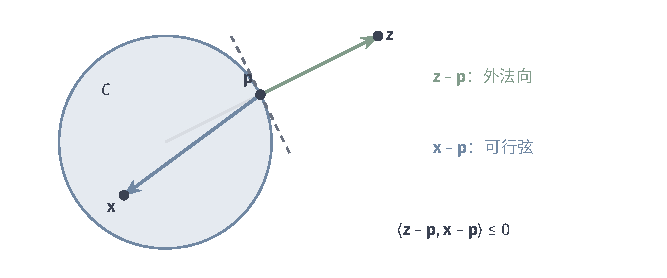
\includegraphics[width=112mm]{figures/01-mathematical-preliminaries-upper/01-mathematical-language-combinatorics-analysis-optimization/tikz/comprehension-additions/projection-normal.pdf}
  \caption{取闭单位圆盘$C$、外点$\bm z=(2,1)^\top$，投影为$\bm p=\bm z/\|\bm z\|_2$。绿箭头$\bm z-\bm p$沿外法向，蓝箭头$\bm x-\bm p$是任一可行弦，内积$\langle\bm z-\bm p,\bm x-\bm p\rangle\leq0$。图中一个参照点仅用于展示。}
  \label{fig:vol1-add-projection-normal}
\end{figure}

盒约束投影逐坐标截断，成本$O(d)$。概率单纯形$\Delta=\{\bm w:w_j\geq0,\sum_jw_j=1\}$不能逐坐标截断，其投影具有共同阈值形式$p_j=\max\{z_j-\tau,0\}$：先排序，再确定正坐标集合，由总和定$\tau$，常用实现$O(d\log d)$。一般凸集的投影本身可能是昂贵子问题。

\subsection{欧氏投影梯度的更新与实现}

把光滑一阶模型加欧氏距离项、只在$C$内最小化，配方得到
\begin{equation}
 \bm w^{(t+1)}
 =\Pi_C\!\left(\bm w^{(t)}-\eta^{(t)}\nabla f(\bm w^{(t)})\right).
 \label{eq:opt-projected-gradient}
\end{equation}
从可行初值出发，输出恒属于$C$。在包含候选与比较线段的开凸域上要求$f$为$L$光滑、取$0<\eta\leq1/L$；未知$L$时按光滑上界回溯，试探要重新求投影。停止量为
\[
 \frac{\|\bm w-\Pi_C(\bm w-\eta\nabla f(\bm w))\|_2}{\eta}
\]
连同原始可行性一起核验。在共同二次目标上取$C=[1,2]\times[0,2]$，$\eta=0.1$时第一步先到梯度中心$(1.8,-1.2)$再投影为$(1.8,0)$；约束最小点$(1,0)$的普通梯度为$(1,0)\neq\bm0$。

\subsection{固定度量的投影梯度变体}

与固定预条件$\bm P\succ\bm0$组合时，投影要匹配距离：
\[
 \bm w^+=\arg\min_{\bm u\in C}
 \|\bm u-(\bm w-\eta\bm P\nabla f(\bm w))\|_{\bm P^{-1}}^2.
\]
其固定点条件消去$\bm P^{-1}\bm P$后恢复原问题的可行一阶条件；若误用欧氏投影截回预条件中心，固定点一般变成$\langle\bm P\nabla f(\bm w),\bm u-\bm w\rangle\geq0$，不等于原条件。对角$\bm P$加盒约束仍逐坐标可分，单纯形或一般耦合$\bm P$须求解新加权最近点问题，不能按原投影成本计费。

\subsection{边界停止与原始目标差}

由式~\eqref{eq:opt-projection-normal}，投影固定点等价于可行一阶条件
\[
 \langle\nabla f(\bm w),\bm v-\bm w\rangle\geq0
 \quad\text{对所有 }\bm v\in C.
\]
若$f$凸，一阶凸下界使该条件足以给原域全局最优；非凸时它只是可行一阶条件。凸$L$光滑、最小点存在、$0<\eta\leq1/L$时，邻近梯度的三点不等式直接给投影迭代目标差$O(1/T)$。

\subsection{梯度与投影误差的传播}

精确映射$T_t(\bm w)=\Pi_C(\bm w-\eta_t\nabla f(\bm w))$；实际梯度读数为$\nabla f(\widetilde{\bm w}^t)+\bm e_t$，含误差中心的精确投影为$\bm p_t$，实际输出满足$\|\widetilde{\bm w}^{t+1}-\bm p_t\|\leq\zeta_t$。投影非扩张给
\[
 \delta_{t+1}\leq\rho_t\delta_t+\eta_t\|\bm e_t\|+\zeta_t,
\]
其中仅$L$光滑时可取$\rho_t=1+\eta_t L$；凸且$L$光滑、$0<\eta_t\leq2/L$时取$1$；再加强凸与$0<\eta_t\leq1/L$时可取$1-\eta_t\mu$。距离误差$\zeta_t$不自动保证输出严格属于$C$，须同时检查实际可行性；实际停止读数与真实投影梯度映射之差不超过$\|\bm e_t\|+\zeta_t/\eta_t$，步长很小时会放大投影计算误差。

\section{惩罚法}

投影难求时，可以允许暂时不可行，把违反量折算进目标。

\subsection{二次惩罚法}

\subsubsection{构造与内外层执行}

二次惩罚目标为
\[
 f+\frac{\rho}{2}\left(\sum_j a_j^2+\sum_k[g_k]_+^2\right).
\]
$[t]_+^2$的导数为$2[t]_+$，故在$f$与约束连续可微时罚项连续可微；约束仿射时还凸且梯度Lipschitz，一般非线性约束（如$a(x)=x^2-1$的平方$(x^2-1)^2$）两项都不继承。执行时先固定$\rho$，核验罚目标结构并选第11—12章的求解器，内层分别报告原目标、违反量与求解精度；外层逐步增大$\rho$，不能仅凭罚目标小梯度停机。

\subsubsection{可行极限与罚参数代价}

对共同目标加等式$w_1+w_2=1$，解驻点方程得
\[
 \bm w_\rho=\frac{(16\rho,\rho)^\top}{16+17\rho},\qquad
 w_1+w_2-1=-\frac{16}{16+17\rho}.
\]
任何有限$\rho>0$仍不可行，极限才是$(16/17,1/17)$。罚Hessian为$\operatorname{diag}(1,16)+\rho\bm1\bm1^\top$，最大特征值随$\rho$趋于无穷，固定步长上限$2/\lambda_{\max}$缩小；最小特征值从$1$增至$17/2$，条件数并非单调变化（$\rho=0,1,225/34$各阶段方向不同），不能只凭最大曲率增大断言持续恶化。

图~\ref{fig:vol1-add-penalty-feasibility-curvature}的两个解析分面分别衡量残差和曲率。
\begin{figure*}[htbp]
  \centering
  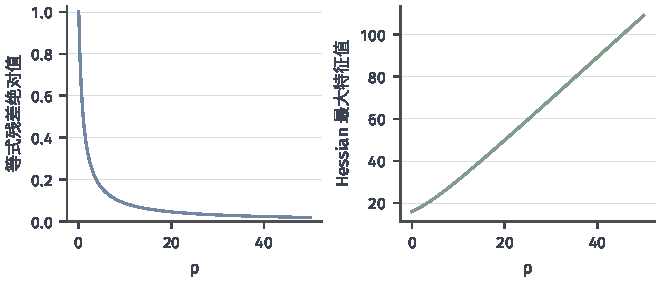
\includegraphics[width=169.0mm]{figures/01-mathematical-preliminaries-upper/01-mathematical-language-combinatorics-analysis-optimization/matplotlib/comprehension-additions/penalty-feasibility-curvature.pdf}
  \caption{共同二次等式加二次惩罚的解析结果。左图约束违反量$16/(16+17\rho)$随$\rho$趋零；右图罚Hessian最大特征值$(17+\sqrt{225+4\rho^2})/2$随$\rho$增大。两图分别衡量可行性与曲率代价，最大特征值不等于条件数。}
  \label{fig:vol1-add-penalty-feasibility-curvature}
\end{figure*}

极限结论需要三个条件各管一段：设违反量$P\geq0$连续、$P=0$恰表可行，$f$下半连续且在候选区域有统一下界$m$，存在可行$\bar{\bm w}$，$\bm w_\rho$精确最小化$f+\rho P$，则与$\bar{\bm w}$比较给$\rho P(\bm w_\rho)\leq f(\bar{\bm w})-m$，违反量随$\rho\to\infty$趋零；再有有界子列才取得极限点；由$P$连续得极限可行，再与任意可行点比较、用下半连续性得极限全局最优。内层近似求解（次优差$\varepsilon_\rho$）时违反量趋零需$\varepsilon_\rho/\rho\to0$。

\subsection{精确惩罚法}

绝对残差
\begin{equation}
 V(\bm w)=\sum_j|a_j(\bm w)|+\sum_k[g_k(\bm w)]_+
 \label{eq:opt-exact-penalty}
\end{equation}
在约束成立时恰为零，罚目标$f+\rho V$通常非光滑，可用第12章的次梯度或邻近方法（但$|a_j(\bm w)|$一般不能逐坐标软阈值）。有限$\rho$能保持原最小解，有两种独立依据。

\paragraph{由可行修复误差界。}
设比较区域$D$含候选及其可行修复，$f$在$D$上$K$-Lipschitz，每个$\bm w\in D$有可行$\bm p\in D$使$\|\bm p-\bm w\|_2\leq\kappa V(\bm w)$，则
\[
 f(\bm w)+\rho V(\bm w)
 \geq f(\bm p)+(\rho-K\kappa)V(\bm w).
\]
$\rho>K\kappa$时不可行点严格劣于其修复点，区域内罚最优解必可行。

\paragraph{由达到的最优乘子。}
若凸约束问题原、对偶均达到且零间隙，取$\rho>\max\{\|\bm\nu^\star\|_\infty,\|\bm\alpha^\star\|_\infty\}$，绝对／正部罚项不小于最优Lagrangian，并对任何非零违反多出严格正量。共同等式例$\nu^\star=-16/17$，故$\rho>16/17$的绝对值惩罚已经精确，与二次惩罚只能在极限可行形成对照。

\subsection{范数惩罚与硬范围的解对应}

硬约束$\|\bm w\|_1\leq R$规定允许范围，正则项$\lambda\|\bm w\|_1$按规模计价，二者不同。若原问题有原始最优解、强对偶成立且有限乘子$\lambda^\star$达到，则原最优解同时最小化$f+\lambda^\star\|\bm w\|_1$（常数$-\lambda^\star R$不改变最小点）；仅有值相等不保证乘子存在。反方向，若$\widehat{\bm w}$最小化$f+\lambda\|\cdot\|_1$，令$R=\|\widehat{\bm w}\|_1$，它也最小化半径$R$的约束问题，但这只构造匹配半径，不证明$\lambda$与$R$一一对应，非凸时还可能有对偶间隙。普通欧氏GD下$f+\lambda\|\bm w\|_2^2/2$的更新为$(1-\eta\lambda)\bm w-\eta\nabla f$；加预条件$\bm P$后正则项走$-\eta\lambda\bm P\bm w$，与独立衰减$-\eta\lambda\bm w$只在匹配条件下相同。

图~\ref{fig:opt-proximal-comparison}比较同一标量输入下投影、软阈值与二次收缩。
\begin{figure}[!htb]
  \centering
  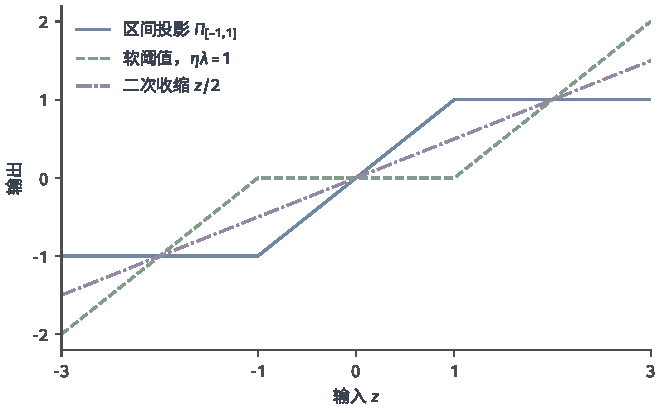
\includegraphics[width=112.0mm]{figures/01-mathematical-preliminaries-upper/01-mathematical-language-combinatorics-analysis-optimization/matplotlib/opt-proximal-comparison/figure.pdf}
  \caption{同一输入$z$的三种邻近映射。区间投影把值截到边界，软阈值把小幅值置零，二次惩罚按比例缩小。}
  \label{fig:opt-proximal-comparison}
\end{figure}

\section{投影对偶上升法}

\subsection{内层求解与乘子更新}

合记乘子$\bm y=(\bm\nu,\bm\alpha)$、允许域$Y=\mathbb R^m\times\mathbb R_+^p$。每轮固定乘子求Lagrangian内层最小点，以约束残差更新价格：
\begin{equation}
 \begin{aligned}
 \bm w^{(t)}&\in\arg\min_{\bm w}\mathcal L(\bm w,\bm y^{(t)}),\\
 \bm s^{(t)}&=(\bm a(\bm w^{(t)}),\bm g(\bm w^{(t)})),\\
 \bm y^{(t+1)}&=\Pi_Y(\bm y^{(t)}+\eta^{(t)}\bm s^{(t)}).
 \end{aligned}
 \label{eq:opt-dual-ascent}
\end{equation}
等式乘子直接加残差，不等式乘子截到非负；违反预算使价格上升，有余量使价格下降。先完整取得内层输出再更新乘子，新旧乘子不能混用。

\subsection{残差方向、步长与对偶目标差}

对任意$\bm y'\in Y$，把当前内层点代入有
\[
 q(\bm y')\leq q(\bm y^{(t)})
 +\langle\bm s^{(t)},\bm y'-\bm y^{(t)}\rangle,
\]
即$q$凹、残差是其全局仿射上界斜率，更新等价于对凸函数$-q$作投影次梯度下降。在最优乘子存在、初始距离$\leq R_y$、残差范数$\leq G_y$下，
\[
 d^\star-\max_{t<T}q(\bm y^{(t)})
 \leq\frac{R_y^2+G_y^2\sum_{t<T}(\eta^{(t)})^2}
 {2\sum_{t<T}\eta^{(t)}},
\]
常步长$\eta=R_y/(G_y\sqrt T)$给$R_yG_y/\sqrt T$。它控制已访问下界，不保证每轮$q$上升，也不控制内层点可行性。

若固定闭凸域上$f$为$\mu$强凸、约束仿射为$\bm A\bm w-\bm b$且内层唯一解达到，则$\bm w(\bm y)$是Lipschitz映射（常数$\|\bm A\|_2/\mu$），两组内层解夹住$q$的增量可证$q$可微且
\[
 \nabla q(\bm y)=\bm A\bm w(\bm y)-\bm b,\qquad
 L_q=\|\bm A\|_2^2/\mu,
\]
从而回用投影梯度的$O(1/T)$光滑界；$\bm A=\bm0$时梯度恒定，取任意正上界。一般非线性约束或多解内层不能直接套用。

\subsection{近似内层的执行、误差与可信下界}

近似内层点须有可信证书$\mathcal L(\widetilde{\bm w}^{(t)},\bm y^{(t)})\leq q(\bm y^{(t)})+\epsilon^{(t)}$；只用其残差更新时，仿射上界多出$\epsilon^{(t)}$，累计目标差界分子增加$2\sum_t\eta^{(t)}\epsilon^{(t)}$，且必须对实际参与更新的近似残差核验有界。近似内层值本身在$q$上方，可信下界应为
\[
 \mathcal L(\widetilde{\bm w}^{(t)},\bm y^{(t)})-\epsilon^{(t)}\leq q(\bm y^{(t)}),
\]
不能直接把内层值充作原问题下界。

\subsection{原始可行恢复与上下界证书}

在预算例（固定$\tau=2$，只对总预算设乘子）中，内层解$\bm w(\alpha)=((2-\alpha)_+,(1-\alpha)_+)^\top$，$q(\alpha)=\alpha-\alpha^2$；取$\alpha^{(0)}=0$、$\eta=1/4$，有$\alpha^{(t)}=\frac12(1-2^{-t})$，前三轮内层点$(2,1),(7/4,3/4),(13/8,5/8)$全部超预算，违反量为$1,1/2,1/4$，而$q$趋于$1/4$。本例两坐标恒正，各减一半预算残差即修复为$(3/2,1/2)$、$U=1/4$；这种简单恢复依赖本例结构，一般问题需独立的投影或恢复算法。即使乘子最优，任意内层点也未必是原解：资源LP对偶例的最优价格处Lagrangian对所有非负分配同值，选$(10,10)$不可行、选$(0,0)$可行却非最优。

\section{对偶分解法}

\subsection{复制变量与独立内层}

对$\min_{\bm w}\{r(\bm w)+s(\bm w)\}$引入两个副本，改写为
\[
 \min_{\bm u=\bm v}\{r(\bm u)+s(\bm v)\}.
\]
一致性等式使两题可行目标相同，复制只改变计算位置。固定等式乘子$\bm\nu$，两个内层独立求解：
\begin{equation}
 \begin{aligned}
 \bm u^{(t)}&\in\arg\min_{\bm u}\{r(\bm u)+\langle\bm\nu^{(t)},\bm u\rangle\},\\
 \bm v^{(t)}&\in\arg\min_{\bm v}\{s(\bm v)-\langle\bm\nu^{(t)},\bm v\rangle\},\\
 \bm\nu^{(t+1)}&=\bm\nu^{(t)}+\eta^{(t)}(\bm u^{(t)}-\bm v^{(t)}).
 \end{aligned}
 \label{eq:opt-consensus-dual-decomposition}
\end{equation}
取齐本轮副本后才算残差、更新乘子；局部副本可暂时不一致，改进的是对偶下界，原目标不保证逐轮下降。

\subsection{强凸与仅凸内层的步长依据}

若$r,s$分别为$\mu_r,\mu_s$强凸，线性项不改变曲率，两个内层解各有$1/\mu_r$、$1/\mu_s$的响应界，残差$\bm u(\bm\nu)-\bm v(\bm\nu)$的Lipschitz常数不超过$1/\mu_r+1/\mu_s$，据此可证对偶可微并选步长；仅凸时回用有界残差的次梯度累计界。子问题无下界或不达到时分解不能直接执行。

\subsection{副本轨迹、一致性与可行证书}

取$r(u)=(u-1)^2/2$、$s(v)=(v+1)^2/2$，内层解为$u=1-\nu$、$v=\nu-1$，$q(\nu)=2\nu-\nu^2$；$\nu^{(0)}=0$、$\eta=1/4$给$\nu^{(t)}=1-2^{-t}$、$u^{(t)}=2^{-t}$、$v^{(t)}=-2^{-t}$。第一轮副本差为$2$，第三轮差$1/2$；平均为$w=0$恢复可行上界$r(0)+s(0)=1$，与下界$q=1-4^{-t}$的间隙为$4^{-t}$。平均恰好最优来自对称二次结构，不是通用恢复规则。

\section{有约束问题的最优性与全局证书}

\subsection{局部最优候选何时满足KKT}

\paragraph{线性化为何可能失真。}
约束$x^2\leq0$在零点的线性化允许所有方向，真实可行集却只有单点，说明没有\term{约束资格条件}时一阶模型推不出乘子。

\paragraph{仿射等式的正交分解。}
对$\bm A\bm w=\bm b$，真实可行扰动满足$\bm A\bm d=\bm0$；局部最优点不能沿$\bm d$与$-\bm d$下降，故$\nabla f(\bm w^\star)\perp\ker\bm A$。由$(\ker\bm A)^\perp=\operatorname{range}(\bm A^\top)$得存在$\bm\nu$使$\nabla f+\bm A^\top\bm\nu=\bm0$，等式乘子无符号限制。共同二次等式例解出$\bm w^\star=(16/17,1/17)^\top$、$\nu=-16/17$。

图~\ref{fig:vol1-add-kkt-normal-balance}展示法向平衡。
\begin{figure}[!htb]
  \centering
  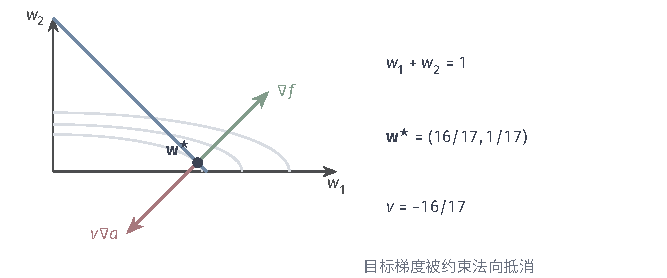
\includegraphics[width=112mm]{figures/01-mathematical-preliminaries-upper/01-mathematical-language-combinatorics-analysis-optimization/tikz/comprehension-additions/kkt-normal-balance.pdf}
  \caption{最小化$(w_1^2+16w_2^2)/2$约束$w_1+w_2=1$。蓝线为可行直线，灰线等值线，在$(16/17,1/17)$处$\nabla f=(16/17,16/17)$，$\nu\nabla a=(-16/17,-16/17)$，等长反向；箭头长度对应法向贡献。}
  \label{fig:vol1-add-kkt-normal-balance}
\end{figure}

\paragraph{LICQ下的必要性。}
设$f,a_j,g_k$在点附近$C^1$且全部等式与活跃不等式梯度线性无关。把这些梯度行扩充为$\mathbb R^d$的一组基，辅以线性坐标$\bm z$构造映射$\bm T(\bm w)=(\bm a(\bm w),\bm g_I(\bm w),\bm z(\bm w))$，由隐函数定理得局部可逆坐标变换；新坐标中可行域恰为$\bm a=0,\bm g_I\leq0$、$\bm z$自由。局部最优令自由坐标偏导为零、活跃不等式坐标偏导非正，链式法则回到原坐标即逐项给出驻点性、非负性与互补松弛。$f(x)=x$、$x^2\leq0$的驻点式$1=0$无解，说明无资格条件时乘子可能不存在。

\subsection{什么证书足以认证全局最优}

若$f$与$g_k$可微凸、$a_j$仿射，且已找到满足全部KKT的候选，对任意可行点应用一阶凸下界并用驻点、等式变化为零、不等式一阶下界与非负乘子，余项非负，即得全局最优。该充分性不需要LICQ或Slater——资格条件解决的是乘子存在性，候选已带乘子时只看凸结构；非凸例$f(x)=-x^2$在零点满足驻点却是极大点。预算例（例~\ref{ex:opt-kkt-budget}）逐区给出KKT解与零乘子切换点，说明活跃不等于正价格；任何情况下，式~\eqref{eq:opt-duality-certificate}的合法上下界不依赖强对偶就能控制目标差。

\begin{example}[活跃约束与预算例]
\label{ex:opt-scalar-active-constraint}
对$\min(x-2)^2/2$、$x\leq a$，$x^\star=\min\{2,a\}$，乘子$u^\star=(2-a)_+$。
\end{example}

\begin{example}[非负预算分配]
\label{ex:opt-kkt-budget}
求最接近$\bm c=(2,1)^\top$的非负分配：
\[
 \min_{\bm w}\frac12\|\bm w-(2,1)^\top\|_2^2
 \quad\text{s.t.}\quad w_1+w_2\leq\tau,\ -w_1\leq0,\ -w_2\leq0.
\]
$\tau>3$时解$(2,1)^\top$，预算不活跃；$\tau=3$时约束活跃但乘子为零；$1<\tau<3$时解$((\tau+1)/2,(\tau-1)/2)^\top$，预算乘子$(3-\tau)/2$；$0<\tau<1$时解$(\tau,0)^\top$，预算乘子$2-\tau$、第二非负约束乘子$1-\tau$。
\end{example}

\subsection{零间隙与最优证书何时达到}

\subsubsection{线性规划强对偶}

先有Farkas择一证书：$\bm M\bm x=\bm r,\bm x\geq\bm0$与$\bm M^\top\bm z\geq\bm0,\bm r^\top\bm z<0$恰有一个可行（两式内积即给矛盾；不可行方向由闭有限生成锥的分离证明）。对标准型
\[
 \min_{\bm x\geq\bm0,\bm A\bm x=\bm b}\bm c^\top\bm x,\qquad
 \max_{\bm A^\top\bm y\leq\bm c}\bm b^\top\bm y,
\]
若原问题可行且下确界$p^\star$有限：可行目标像为一维下有界多面体、含自己的有限下端点，故原始最优达到；对每个$\varepsilon>0$把“目标值$p^\star-\varepsilon$”加入不可行系统，由Farkas构造对偶可行点其值大于$p^\star-\varepsilon$，再由对偶目标像为上端封闭的一维多面体知对偶最优达到且同值。

\begin{example}[二维资源分配]
\label{ex:opt-resource-lp-duality}
$\max_{x_1,x_2\geq0}3x_1+2x_2$，约束$2x_1+x_2\leq4$、$x_1+2x_2\leq4$。原始点$(4/3,4/3)$与对偶点$(u_1,u_2)=(4/3,1/3)$的值均为$20/3$，弱对偶即认证两者同时最优。
\end{example}

沿可行射线无界改善时，弱对偶只说明每个允许乘子的$q$都是$-\infty$（标准型中表现为对偶不可行），不意味着乘子允许域为空；只有下确界不达到则展示不出原始最优点。

\subsubsection{Slater资格}

为处理低维定义域，定义\term{仿射包}$\operatorname{aff}C$（权重可为负、和为$1$的有限仿射组合）与\term{相对内部}$\operatorname{ri}D$：存在$r>0$使$B(\bm x,r)\cap\operatorname{aff}D\subseteq D$。平面线段无二维内部，但去端点线段是其相对内部。

\begin{theorem}[Slater条件下的强对偶]
设$f$与不等式函数$g_k$为适当凸函数、具有共同凸有效定义域$D$，等式为仿射约束，存在$\bar{\bm w}\in\operatorname{ri}D$满足$\bm A\bar{\bm w}=\bm b$和所有$g_k(\bar{\bm w})<0$，且原最优值有限，则原、对偶最优值相等且存在最优对偶乘子。
\end{theorem}

其一般证明需要凸集的一般分离及扰动值集合（未必闭）的边界处理，本章陈述并准确引用，不伪装成已完整证明。Slater不保证原始最小点达到：$\min_x e^x$最优值$0$而无最优点；反过来，已找到KKT候选时其全局充分性不需要Slater。预算例同时具备可行、原始达到（闭域强制）、零间隙与对偶达到，这四件事须分别核验。\term{凸共轭}提供了计算某些仿射约束对偶值的工具（例如单一等式约束可用共轭算下界），但共轭可算、值达到、乘子达到仍是不同问题；Fenchel--Moreau定理说明闭凸函数恰为其全部仿射下界的上包络。

\section{收敛速度与计算预算的比较}

凸光滑原始目标与非空闭凸可行域上，投影梯度给$O(1/T)$原始目标差；对偶光滑且乘子达到时$d^\star-q$同为$O(1/T)$，非光滑残差按次梯度累计界评价；即使零间隙，实际全局证书仍用独立恢复的$U-q$。二次罚的参数极限结论不是按外层次数的速率，精确罚还要看内层方法的实际精度。停止时先报告实际违反量，再报告合法下界与可行上界之差；预算例残差按$2^{-t}$、间隙按$4^{-t}$缩小，依赖特定二次结构与步长。总预算要合计外层迭代、梯度／残差求值、投影或内层求解成本，不能只比外层次数。

\section{误差传播与约束参数敏感性}

\subsection{计算误差怎样影响轨迹与停止}

投影轨迹误差按13.2.5传播；近似对偶内层的累计项与可信下界按13.4.3进入；罚方法比较式控制的是违反量。数值残差应分项报告：即使无约束凸目标，梯度$\delta$在$f(x)=\epsilon x^2/2$下对应目标差$\delta^2/(2\epsilon)$，小KKT残差脱离尺度不构成目标差证书，全局差距仍由式~\eqref{eq:opt-duality-certificate}承担。

\subsection{约束参数怎样改变最优解}

\paragraph{内点分支。}
对依赖$\theta$的无约束目标，驻点方程$\varphi_z(z,\theta)=0$在$\varphi_{zz}\neq0$时由隐函数定理给出局部分支；例$\varphi(z,\theta)=\frac12(1+\theta)z^2-\theta z$（$\theta>-1$）的解$z^\star=\theta/(1+\theta)$，导数$1/(1+\theta)^2$可由隐式与显式两种方式复算，但分支是否全局最优仍要另行核验。

\paragraph{固定活跃集的KKT系统。}
固定活跃集$I$，把驻点、等式与活跃不等式等号条件写成$\bm\Phi(\bm w,\bm\nu,\bm\alpha_I,\tau)=\bm0$。Jacobian可逆时局部解连续可微；所需的是完整KKT块矩阵
\[
 \begin{bmatrix}
 \nabla_{\bm w,\bm w}^2\mathcal L&\bm A_I^\top\\
 \bm A_I&\bm0
 \end{bmatrix}
\]
可逆，原目标Hessian可逆并不足够。若$\bm A_I$满行秩且Lagrangian Hessian在$\ker\bm A_I$上正定，齐次方程先逼方向进核、再内积逼其为零，块矩阵可逆；活跃乘子严格为正与未活跃严格余量使小邻域保持同一活跃集。预算例$1<\tau<3$时解导数$(1/2,1/2)^\top$、$0<\tau<1$时$(1,0)^\top$，$\tau=1$解连续但导数改变。

\subsection{约束参数怎样改变最优值}

内点驻点使链式法则中含解导数的项消失：$V'(\theta)=\partial\varphi/\partial\theta|_{z=z^\star}$，这是\term{包络定理}的基本机制，但解导数本身仍存在。约束写成$g_k(\bm w)-\tau_k\leq0$时，对保持全局最优的分支，
\[
 \frac{\partial V}{\partial\tau_k}=-\alpha_k^\star
\]
（未活跃乘子取零）；只有该分支继续全局最优（凸问题中KKT充分性保证这一点），局部分支值才等于全局最优值。预算例值函数
\[
 V(\tau)=
 \begin{cases}
 0,&\tau\geq3,\\
 (3-\tau)^2/4,&1\leq\tau\leq3,\\
 ((2-\tau)^2+1)/2,&0<\tau\leq1
 \end{cases}
\]
逐区间满足$V'(\tau)=-\alpha_{\rm bud}^\star$；放宽预算$\Delta\tau$的一阶收益是$\alpha^\star\Delta\tau$，这是值变化率而非参数移动量。

图~\ref{fig:opt-budget-active-set}沿同一预算轴展示解坐标与乘子。
\begin{figure*}[htbp]
  \centering
  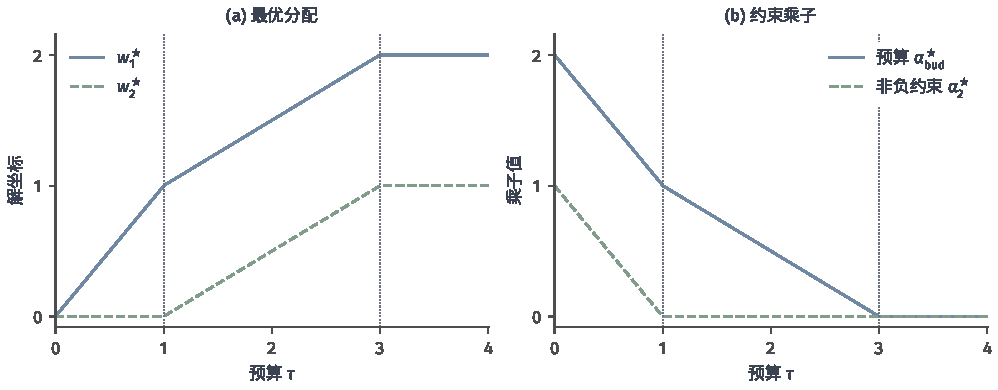
\includegraphics[width=169.0mm]{figures/01-mathematical-preliminaries-upper/01-mathematical-language-combinatorics-analysis-optimization/matplotlib/opt-budget-active-set/figure.pdf}
  \caption{例~\ref{ex:opt-kkt-budget}的解析解。左图为两个最优分配坐标，右图为预算乘子与第二非负约束乘子。竖线标出$\tau=1,3$；切换点约束可取等号而乘子为零。}
 \label{fig:opt-budget-active-set}
\end{figure*}

\section{本章小结}

三条约束路线各改一个计算对象：投影保持落点可行，惩罚通过违反量改变比较目标，乘子与对偶建立梯度平衡和下界。它们可以组合，但每次组合都要重新写清内层域、被对偶化的约束与实际目标。证书分三层：LICQ支持局部KKT必要性，凸结构支持KKT候选的全局充分性，合法下界配合可行上界直接控制目标差；Farkas认证线性不可行，LP强对偶与Slater分别给出不同结构上的零间隙依据，任何一项都不能替代全部达到性核验。残差驱动的对偶更新改善下界，内层点仍需恢复原始可行，近似内层误差必须进入累计界与可信下界；最优值对约束参数的变化率由活跃乘子给出，且依赖活跃集、完整KKT系统与分支全局最优。
